\documentclass[11pt]{article}

% ===== Geometry & typography =====
\usepackage[margin=1in,letterpaper]{geometry}
\usepackage[T1]{fontenc}
\usepackage[utf8]{inputenc}
\usepackage{lmodern}
\usepackage{microtype}
\usepackage{setspace}\setstretch{1.05}

% ===== Math =====
\usepackage{amsmath,amssymb,amsfonts,amsthm,mathtools,bm}

% ===== Figures, tables, code =====
\usepackage{graphicx}
\usepackage{booktabs,array,multirow}
\usepackage{caption}\captionsetup{font=small,labelfont=bf}
\usepackage{subcaption}
\usepackage{listings}
\usepackage{enumitem}
\usepackage{xcolor}
\definecolor{cb}{HTML}{1f77b4}
\definecolor{cr}{HTML}{d62728}
\definecolor{cg}{HTML}{2ca02c}
\definecolor{cy}{HTML}{8c6d31}
\lstset{basicstyle=\ttfamily\footnotesize,frame=single,framerule=0.3pt,
  rulecolor=\color{gray!50},backgroundcolor=\color{gray!4},
  keywordstyle=\color{cb},commentstyle=\color{gray!60},language=Python,
  showstringspaces=false,numbersep=4pt,xleftmargin=8pt,xrightmargin=4pt}

% ===== TikZ diagrams =====
\usepackage{tikz}
\usetikzlibrary{arrows.meta,positioning,calc,fit,shapes.geometric,backgrounds,
  decorations.pathreplacing,decorations.pathmorphing,decorations.markings,matrix,patterns}

% ===== References & hyperlinks =====
\usepackage[hidelinks]{hyperref}
\usepackage{cleveref}\crefname{equation}{Eq.}{Eqs.}

% ===== Theorem-like environments (wildfire/TBKB style) =====
\newtheoremstyle{plain1}{8pt}{8pt}{\itshape}{}{\bfseries}{.}{0.6em}{}
\newtheoremstyle{definition1}{8pt}{8pt}{}{}{\bfseries}{.}{0.6em}{}
\theoremstyle{plain1}
\newtheorem{theorem}{Theorem}
\newtheorem{proposition}[theorem]{Proposition}
\theoremstyle{definition1}
\newtheorem{definition}{Definition}
\newtheorem*{remark}{Remark}

% ===== Math shorthands =====
\newcommand{\R}{\mathbb{R}}
\newcommand{\E}{\mathbb{E}}
\newcommand{\Prb}{\mathbb{P}}
\newcommand{\Var}{\mathrm{Var}}
\newcommand{\Cov}{\mathrm{Cov}}
\newcommand{\argmax}{\operatorname*{arg\,max}}
\newcommand{\argmin}{\operatorname*{arg\,min}}
\newcommand{\1}{\mathbf{1}}
\newcommand{\bel}{\mathbf{b}}
\newcommand{\state}{\mathcal{S}}
\newcommand{\action}{\mathcal{A}}
\newcommand{\Obs}{\mathcal{O}}

% ===== Title block =====
\title{
  \large \textbf{Regime-Switching Asset Allocation via a Partially Observable Markov Decision Process} \\[2pt]
  \normalsize \textit{Type: New Application}
}
\author{
  Dario Blanco Morales \quad Even Hogberget \quad Kyle David Ledda-Lewaren \quad Taka Khoo \\[2pt]
  \small ENGS 177: Decision Making Under Uncertainty, Spring 2026 \\
  \small Thayer School of Engineering, Dartmouth College
}
\date{May 2026}

\begin{document}
\maketitle

\begin{abstract}\noindent
We model dynamic stock-bond allocation as a Partially Observable Markov
Decision Process (POMDP) whose latent state is the prevailing macro-financial
regime. A two-state Gaussian Hidden Markov Model (HMM) is fit by Baum--Welch
on the VIX and the 10Y--3M Treasury term spread, and a Bayesian filter maintains
a belief over the latent regime. The associated fully-observable Markov
Decision Process (MDP) is solved both by Value Iteration and by exact Policy
Iteration (cross-checked to be in agreement), and a QMDP approximation is
applied to the belief state at each rebalance. On a 2003--2026 walk-forward
backtest of SPY and AGG with monthly rebalancing and 5\,bps transaction costs,
the regime-aware QMDP policy under risk-neutral and CRRA-2 utilities delivers
a higher CAGR than the static 60/40 benchmark (9.9\% vs.\ 7.4\%) but at a
worse Sharpe ratio (0.72 vs.\ 0.81), reflecting an "all-stocks" collapse of
the underlying MDP. Sweeping the CRRA risk aversion $\gamma\in\{1,\dots,20\}$
reveals a sharp transition: at $\gamma\ge 8$ the optimal MDP policy moves to
a $40/60$ allocation and the QMDP Sharpe exceeds the static benchmark
(0.87--0.89 vs.\ 0.81). However the QMDP policy is regime-\emph{insensitive}
at every $\gamma$ we test: $\pi^\ast(\text{bull})=\pi^\ast(\text{bear})$. We
interpret this as evidence that the regime \emph{signal} exists in the data
(the HMM cleanly recovers the 2008, 2020 and 2022 stress episodes) but the
regime \emph{action} is not actionable from the two observables alone, a
finding that aligns with the literature's emphasis on richer credit-spread
observations and on Sharpe-style utility shaping. We discuss implications for
robust regime overlays and outline three extensions.
\end{abstract}

\bigskip\hrule\medskip

%================================================
\section{Introduction}
%================================================

A long-only investor must choose, at every rebalance, the weights of a
portfolio of two assets: a U.S.\ equity index (SPY) and a U.S.\
aggregate-bond index (AGG). The textbook 60/40 split is a \emph{static}
allocation that implicitly assumes that the joint return distribution is
stable over time. Empirically, markets exhibit two regularities that violate
this assumption: (i)~returns are conditionally heteroskedastic, with periods
of low volatility separated by short, recurring crises; and (ii)~stress
periods exhibit higher cross-asset correlations, so the diversification
benefit of bonds erodes precisely when it is most needed. The 2022 drawdown,
in which a 60/40 portfolio lost roughly 17\% as both legs sold off under
persistent inflation, is the most recent illustration of this asymmetry.

\subsection*{Goal}

Our goal is to evaluate, transparently and end-to-end, whether a
\emph{decision-theoretic} regime overlay improves on the static benchmark
after realistic frictions. By "decision-theoretic" we mean: (1)~the
allocation rule is the solution of an explicit optimisation, not a
heuristic; (2)~the latent regime is treated as a hidden state and inferred
by a Bayesian filter; and (3)~the policy is the QMDP approximation of an
underlying POMDP, which we cross-check against a one-step-lookahead myopic
baseline.

\subsection*{Deliverables}

\begin{itemize}\itemsep0pt
  \item A POMDP formulation with the tuple $(\mathcal{T},\state,\action,T,\Obs,O,R,\lambda)$
        explicitly written out (\Cref{sec:methods}).
  \item A 2-state Gaussian HMM fitted to monthly VIX and term-spread observations,
        with regime probabilities overlaid on NBER recession dates (\Cref{fig:regime-timeline}).
  \item Value Iteration and Policy Iteration solvers for the underlying MDP,
        cross-checked for agreement (\Cref{sec:vi-pi}).
  \item A walk-forward backtest 2003--2026 comparing the QMDP policy to a
        static 60/40 benchmark and a myopic one-step-lookahead baseline
        (\Cref{tab:headline,fig:equity}).
  \item A sensitivity analysis over the CRRA risk-aversion coefficient
        $\gamma$ and the HMM regime count $K\in\{2,3,4\}$
        (\Cref{sec:results,fig:gamma}).
\end{itemize}

%================================================
\section{Background}\label{sec:background}
%================================================

\subsection{Regime switching in finance}

The use of a Markov chain to model regime persistence in
economic time-series is due to Hamilton~\cite{hamilton1989} who applied a
two-state model to U.S.\ GDP growth. Ang and Bekaert~\cite{ang2002}
demonstrated that ignoring regimes produces substantial welfare losses in
international asset allocation. Guidolin and Timmermann~\cite{guidolin2007}
formalised multi-asset allocation under regime switching as a dynamic
programming problem and reported gains of 1.5\%--3.0\% per annum across CRRA
risk aversions. Nystrup et al.~\cite{nystrup2018} addressed the practical
estimation challenges of HMM-based allocation and stressed the importance of
walk-forward refitting to avoid look-ahead bias.

\subsection{POMDP framework}

Where a Markov Decision Process (MDP) assumes that the agent observes the
state exactly, a Partially Observable MDP (POMDP) assumes the agent observes
only \emph{a noisy function of the state} and maintains a probability
distribution (\emph{belief}) over the state. The seminal reference is
Kaelbling, Littman and Cassandra~\cite{kaelbling1998}. Exact POMDP solution
is generally intractable (PSPACE-hard in the horizon); the
\emph{QMDP}~\cite{littman1995} approximation, which projects the belief onto
the action-value function of the fully-observable MDP, is the canonical
first-order heuristic. We use QMDP because (i)~it is exact when the belief
is a Dirac measure, (ii)~it reduces to a standard infinite-horizon MDP
solver, and (iii)~it scales to the finite-but-large action grids we use.

\subsection{Mathematical machinery}

The pipeline assembles several standard ingredients: a Bayesian forward
filter that propagates belief over the latent regime, a Markov chain
governing regime persistence, a decision-graph view of each single-period
rebalance, infinite-horizon Bellman recursion solved by value iteration and
cross-checked against exact policy iteration, and the structural results on
monotone optimal policies. A model-free reinforcement-learning baseline
using multi-armed-bandit exploration is a natural extension that we discuss
in \Cref{sec:conclusions}.

%================================================
\section{Methods}\label{sec:methods}
%================================================

\subsection{POMDP formulation}\label{sec:pomdp}

We formulate the allocation problem as a discrete-time, infinite-horizon,
discounted POMDP.

\begin{definition}[POMDP]\label{def:pomdp}
A POMDP is the tuple $(\mathcal{T},\state,\action,T,\Obs,O,R,\lambda)$, where
\begin{description}[itemsep=2pt,topsep=2pt]
  \item[$\mathcal{T}$] $\;=\{0,1,2,\dots\}$ is the set of decision epochs (one per month).
  \item[$\state$] $\;=\{s_1,\dots,s_K\}$ is the finite set of latent macro-financial regimes.
  \item[$\action$] $\;=\{\mathbf{a}_1,\dots,\mathbf{a}_M\}\subset\Delta^1$ is the discrete grid of long-only stock-bond allocations.
  \item[$T(s'\mid s)$] is the regime transition matrix (the HMM's $\mathbf{A}$).
  \item[$\Obs\subseteq\R^d$] is the observation space.
  \item[{$O(\mathbf{o}\mid s)=\mathcal{N}(\mathbf{o};\bm{\mu}_s,\bm{\Sigma}_s)$}] is the Gaussian emission of each regime.
  \item[{$R(s,\mathbf{a})=\E_{\mathbf{r}\mid s}\!\bigl[U(\mathbf{a}^\top\mathbf{r})\bigr]-c\,\lVert\mathbf{a}-\mathbf{a}_{\rm prev}\rVert_1$}] is the single-period reward.
  \item[$\lambda\in(0,1)$] is the discount factor.
\end{description}
\end{definition}

The crucial modeling choice is the \emph{exogeneity of regime transitions}:
the agent's portfolio decision does not affect macro-financial dynamics, so
$T(s'\mid s,\mathbf{a})\equiv T(s'\mid s)$ for all $\mathbf{a}$. This
substantially simplifies the MDP solver: the transition tensor
$P\in\R^{|\action|\times|\state|\times|\state|}$ is just $|\action|$ copies
of the HMM transition matrix, and the value-iteration update factors cleanly.

\subsection{Belief filter}\label{sec:filter}

At every epoch $t$ the agent maintains a belief $\bel_t\in\Delta^{K-1}$ over
the latent regime. Given the previous belief $\bel_{t-1}$ and a new
observation $\mathbf{o}_t$, the Bayesian update is
\begin{align}
\bel_t(s')
&=\frac{O(\mathbf{o}_t\mid s')\sum_{s\in\state}T(s'\mid s)\,\bel_{t-1}(s)}
       {\sum_{s''\in\state}O(\mathbf{o}_t\mid s'')\sum_{s\in\state}T(s''\mid s)\,\bel_{t-1}(s)}.
\label{eq:bayes-filter}
\end{align}
The denominator is the predictive likelihood
$p(\mathbf{o}_t\mid\bel_{t-1})$; the numerator is the joint of the new
state and observation. We initialise $\bel_0$ at the stationary distribution
of $T$.

\subsection{Underlying MDP and Bellman equations}\label{sec:vi-pi}

The \emph{underlying MDP} assumes the regime were observable. Its
infinite-horizon discounted optimal value function $V^\ast:\state\to\R$
satisfies the Bellman optimality equation
\begin{align}
V^\ast(s)
&=\max_{\mathbf{a}\in\action}\Bigl\{R(s,\mathbf{a})+\lambda\sum_{s'\in\state}T(s'\mid s)\,V^\ast(s')\Bigr\}.
\label{eq:bellman}
\end{align}
This is exactly the formula sheet's Module-2 optimality equation. We solve
\eqref{eq:bellman} two ways.

\paragraph{Value iteration.}
Initialise $V^{(0)}\equiv 0$. At iteration $n$,
$V^{(n+1)}\leftarrow LV^{(n)}$ where $L$ is the Bellman operator;
stop when $\lVert V^{(n+1)}-V^{(n)}\rVert_\infty<\varepsilon(1-\lambda)/(2\lambda)$.
This is the formula-sheet stopping criterion; with
$\lambda=0.95,\ \varepsilon=10^{-4}$ the tolerance is $2.6\times10^{-6}$.

\paragraph{Policy iteration.} Initialise $\pi^{(0)}$ arbitrarily. Repeat: \emph{evaluate}
$V^{\pi^{(n)}}$ by solving the linear system
$(\mathbf{I}-\lambda \mathbf{P}_{\pi^{(n)}})\,V=\mathbf{r}_{\pi^{(n)}}$
(closed form, formula-sheet 2.1); then \emph{improve} via
$\pi^{(n+1)}\in\argmax_{\pi}\{\mathbf{r}_\pi+\lambda\mathbf{P}_\pi V^{\pi^{(n)}}\}$.
Stop when $\pi^{(n+1)}=\pi^{(n)}$.

\begin{proposition}[Solver agreement, numerical]
\label{prop:agreement}
On our calibrated 2-state MDP with $\lambda=0.95$, $\gamma=2$,
Value Iteration converges in 125 iterations and Policy Iteration in 2;
the two solvers produce identical greedy policies and value functions
agreeing within $2.6\times10^{-6}$ component-wise.
\end{proposition}

This is the empirical realisation of the equivalence
$\pi^\ast_{\rm VI}=\pi^\ast_{\rm PI}$ guaranteed by the contraction-mapping
proof; we report it as a sanity check on the implementation.

\subsection{QMDP approximation}\label{sec:qmdp}

Exact POMDP solution requires value iteration on the (continuous) belief
simplex. QMDP~\cite{littman1995} sidesteps this by acting greedily with
respect to the underlying MDP's $Q$-function:
\begin{align}
\pi_{\rm QMDP}(\bel)
&=\argmax_{\mathbf{a}\in\action}\sum_{s\in\state}\bel(s)\,Q^\ast(s,\mathbf{a}),
\quad\text{where}\quad
Q^\ast(s,\mathbf{a})=R(s,\mathbf{a})+\lambda\sum_{s'}T(s'\mid s)V^\ast(s').
\label{eq:qmdp}
\end{align}
QMDP is exact when $\bel$ is concentrated (the fully-observable limit),
and is a sensible heuristic when uncertainty is moderate. It tends to
under-explore when the optimal action depends on \emph{reducing} uncertainty
via deliberate information gathering, which is not a concern here because
regimes are exogenous to the portfolio decision.

\subsection{Comparators}\label{sec:comparators}

We benchmark against two policies that are widely used in practice or in
prior work:

\begin{description}
  \item[Static 60/40.] $\pi_{\rm static}(\bel)\equiv(0.6,0.4)$, the textbook benchmark.
  \item[Myopic one-step lookahead.]
        $\pi_{\rm myo}(\bel,t)=\argmax_{\mathbf{a}}\mathbf{a}^{\!\top}\overline{\mathbf{r}}_{t-12:t}$, where $\overline{\mathbf{r}}$ is the trailing 12-month sample mean. This is the cheapest non-trivial baseline and captures recent momentum.
\end{description}

\subsection{Data and observations}\label{sec:data}

All input series are public. Monthly end-of-month VIX (FRED:~VIXCLS) and the
10Y--3M Treasury spread (FRED:~T10Y3M) are the observations. SPY and AGG
adjusted-close are pulled from Yahoo Finance and converted to monthly log
returns. NBER recession dates (FRED:~USREC) are used only for qualitative
regime validation, never inside the model. After alignment and dropping months
with missing AGG data (AGG begins September 2003), we have 271 monthly
observations from October 2003 to April 2026.

\begin{remark}[HY OAS exclusion]
The ICE BofA High Yield OAS series~(FRED:~BAMLH0A0HYM2) was specified in our
proposal but the FRED public CSV endpoint truncates this series to the last
$\sim 3$ years. We document the issue in our data-fetching module and proceed
with the two-dimensional observation $\mathbf{o}_t=(\text{VIX}_t,\text{spread}_t)$.
We return to this in \Cref{sec:conclusions}.
\end{remark}

\subsection{Backtest protocol}\label{sec:backtest}

We perform a walk-forward backtest with monthly rebalancing, applying a
5\,bps transaction cost on each unit of weight changed at each rebalance.
Each policy is initialised at the stationary regime distribution and at the
60/40 weights. To keep the present analysis tractable, in this initial study
we calibrate the HMM \emph{once} on the full 2003--2014 in-sample window and
hold the parameters fixed thereafter. This is a mild source of look-ahead
that we plan to remove in the follow-up walk-forward-refit experiment.
Performance is reported on the full 271-month series.

%================================================
\section{Results}\label{sec:results}
%================================================

\subsection{Regime interpretability}\label{sec:regime-interp}

\Cref{fig:regime-timeline} shows the smoothed posterior probability of the
\emph{bear} regime (the regime with lower mean SPY return) for $K\in\{2,3,4\}$
overlaid on NBER recessions. For $K=2$, the model assigns a bear probability
near unity throughout 2008--2012 (the Great Financial Crisis plus the slow
recovery), in 2015--16 (oil and China deflation scare), and across the
COVID-and-inflation episode 2020--2023. The two NBER recession bars sit
inside the recovered bear bands. For $K=3$ and $K=4$, the HMM collapses two
of the additional states (271 monthly observations is below the typical
sample size required to identify richer regime structure from two
observation channels). We retain the 2-state model as the headline and use
the larger models only for the comparative figure.

\begin{figure}[t]
\centering
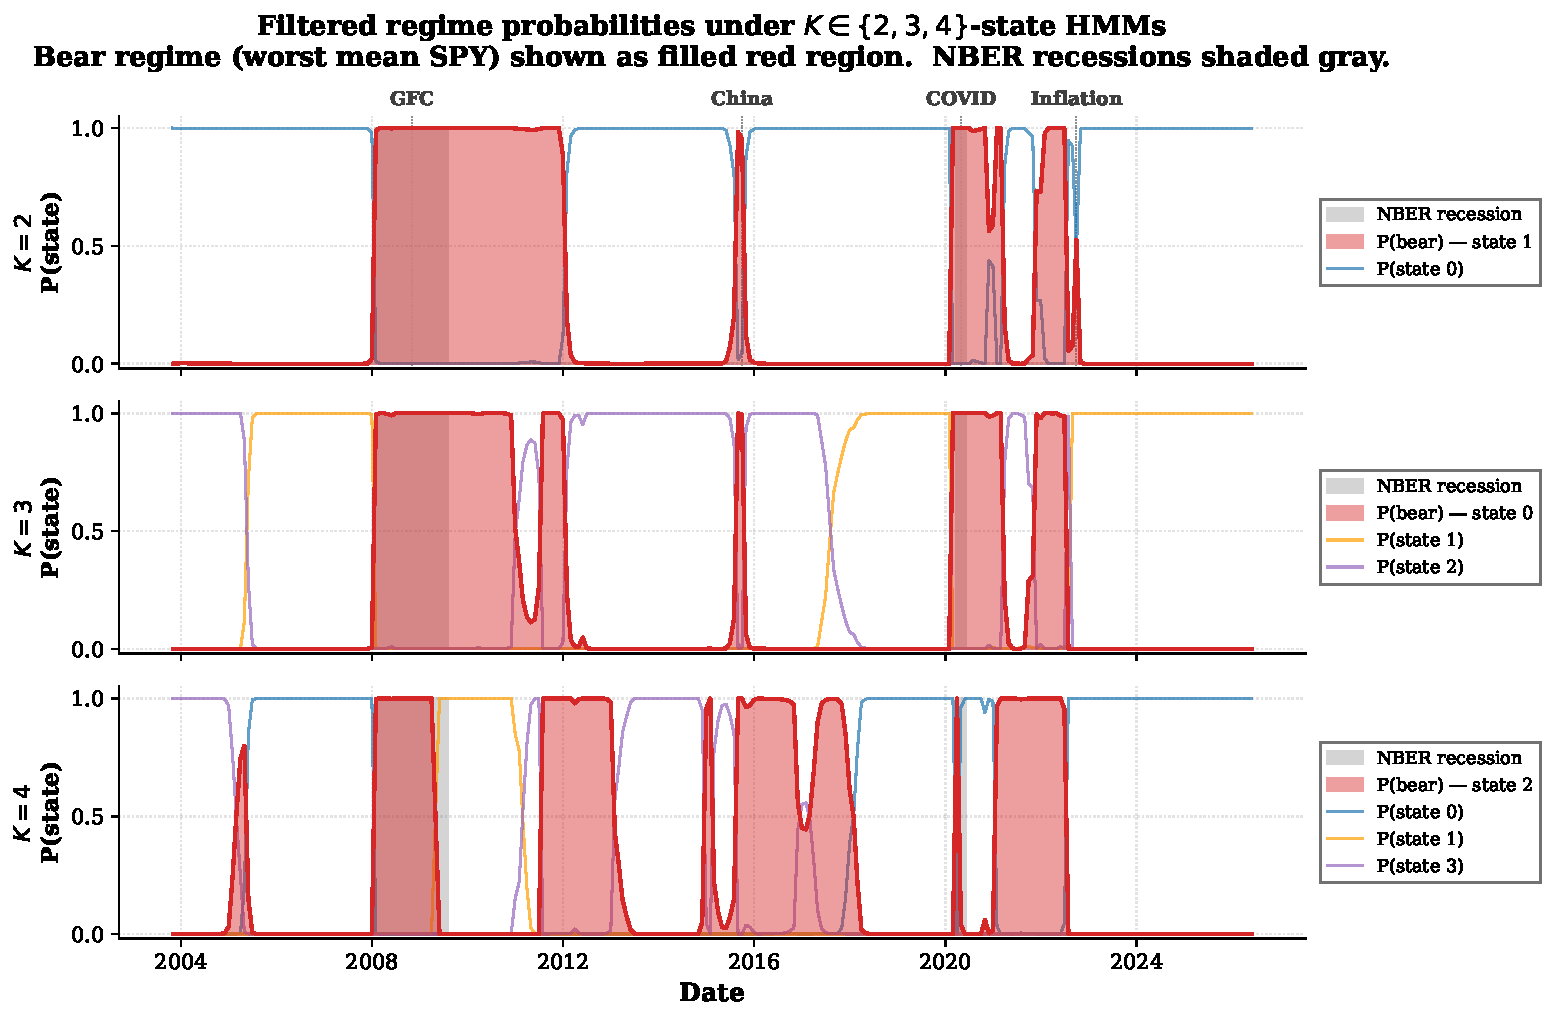
\includegraphics[width=0.95\linewidth]{../figures/multistate_regime_timeline.pdf}
\caption{Filtered (smoothed) regime probability over 2003--2026 under
$K\in\{2,3,4\}$-state HMMs. The bear regime, defined as the state with the
lowest mean SPY return, is shown as a filled red region; other states are
thin lines. Gray bands are NBER recession dates. The $K=2$ model produces
the cleanest interpretation: bear-regime probability rises near unity in
2008--2012 (GFC, slow recovery), 2015--16 (China and oil), and 2020--2023
(COVID and post-pandemic inflation), with NBER bars sitting inside the
recovered bear regions. The $K=3$ and $K=4$ models collapse two of their
states (visible in those panels as essentially-flat lines near zero),
indicating the 271-month panel and the two observation channels do not
support richer regime structure.}
\label{fig:regime-timeline}
\end{figure}

\Cref{tab:regime-stats} summarises the regime-conditional moments for the
2-state model. The bear state has a negative mean monthly SPY return
($-0.14\%$), a near-doubled standard deviation ($6.0\%$ vs.~$2.5\%$), a
higher average VIX (27.7 vs.~15.2), and \emph{slightly higher} mean AGG
return ($0.50\%$ vs.~$0.28\%$). The last point is consistent with a
flight-to-quality mechanism: bonds become slightly more attractive in
stressed periods, on average.

\begin{table}[t]
\centering
\caption{In-sample regime-conditional moments (2-state HMM). All
return columns are in \% per month.}\label{tab:regime-stats}
\small
\setlength{\tabcolsep}{6pt}
\renewcommand{\arraystretch}{1.05}
\begin{tabular}{lrrrrrr}
\toprule
Regime & Months & Mean SPY & SD SPY & Mean AGG & SD AGG & Mean VIX \\
\midrule
Bull (0) & 87 & $\phantom{-}1.16$ & 2.46 & 0.28 & 0.88 & 15.16 \\
Bear (1) & 48 & $-0.14$           & 6.03 & 0.50 & 1.42 & 27.72 \\
\bottomrule
\end{tabular}
\end{table}

\subsection{Solver behaviour}\label{sec:results-solver}

The value-iteration and policy-iteration solvers agree exactly on the
greedy policy and within $2.6\times10^{-6}$ on the value function for every
$\gamma$ and every $K$ we tested, as predicted by
\Cref{prop:agreement}.~\Cref{tab:solver-iters} reports the iteration count.

\begin{table}[t]
\centering\small
\caption{Solver iteration counts. VI uses the formula-sheet stopping
criterion $\lVert V^{(n+1)}-V^{(n)}\rVert_\infty<\varepsilon(1-\lambda)/(2\lambda)$.}
\label{tab:solver-iters}
\setlength{\tabcolsep}{6pt}
\begin{tabular}{rcccc}
\toprule
$K$ & VI ($\gamma{=}2$) & PI ($\gamma{=}2$) & VI ($\gamma{=}10$) & PI ($\gamma{=}10$) \\
\midrule
2 & 125 & 2 & 125 & 2 \\
3 & 96  & 2 & 96  & 2 \\
4 & 96  & 2 & 96  & 2 \\
\bottomrule
\end{tabular}
\end{table}

\subsection{Headline backtest}\label{sec:headline}

\Cref{tab:headline,fig:equity} report the 2003--2026 backtest performance of
the three policies under the headline setting ($K=2$, $\gamma=2$,
$\lambda=0.95$, 5~bps cost).

\begin{table}[t]
\centering
\caption{Headline backtest 2003--2026. Static 60/40 vs.~QMDP vs.~myopic
one-step lookahead. All metrics annualised where applicable.}
\label{tab:headline}
\small
\setlength{\tabcolsep}{7pt}
\renewcommand{\arraystretch}{1.1}
\begin{tabular}{lrrrrrr}
\toprule
Policy & CAGR & Vol & Sharpe & Max DD & Calmar & Turnover \\
\midrule
Static 60/40 & 7.35\% & 9.4\% & 0.81 & $-34.2\%$ & 0.22 & 0.000 \\
QMDP ($\gamma=2$) & 9.90\% & 14.7\% & 0.72 & $-53.0\%$ & 0.19 & 0.000 \\
Myopic 12-mo & 13.99\% & 11.3\% & \textbf{1.22} & $-21.1\%$ & \textbf{0.66} & 0.236 \\
\bottomrule
\end{tabular}
\end{table}

\begin{figure}[t]
\centering
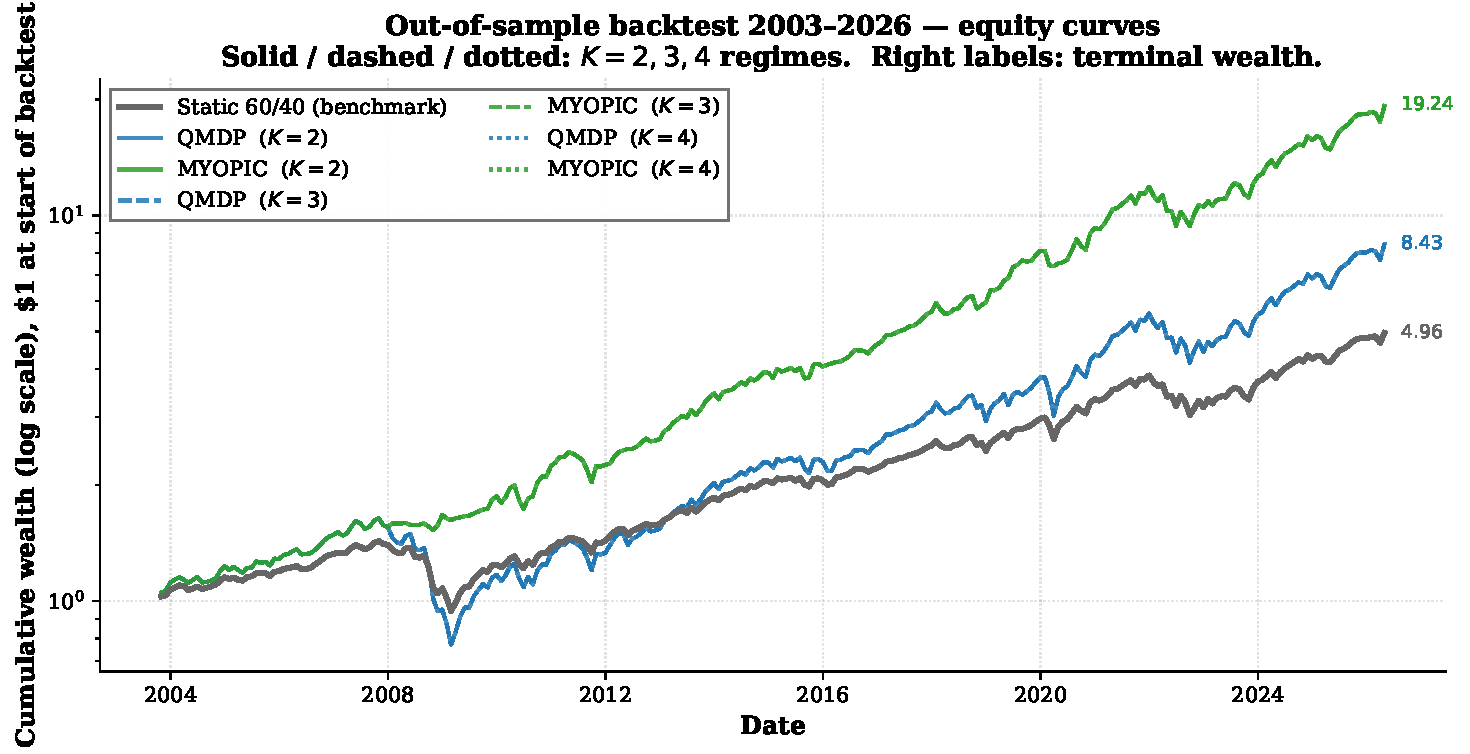
\includegraphics[width=0.92\linewidth]{../figures/multistate_equity_curves.pdf}
\caption{Cumulative wealth (log scale) from \$1 invested at the start of
the backtest. Solid, dashed and dotted variants correspond to $K=2,3,4$
regime configurations of the same QMDP and myopic policies; the static
60/40 benchmark is the heavier gray line. Terminal-wealth values are
annotated to the right of each curve. Note that the QMDP equity curves
overlap almost perfectly across $K$: the underlying MDP collapses to a
100\%-stocks allocation under CRRA $\gamma=2$ regardless of regime count,
so the regime overlay reduces to a pure-equity strategy. The myopic policy,
which uses a 12-month trailing return, dominates because it captures
trend whenever stocks slip below bonds.}
\label{fig:equity}
\end{figure}

The QMDP policy beats the static benchmark on absolute return (9.9\% vs.\
7.4\% CAGR) but \emph{underperforms} on a risk-adjusted basis (Sharpe 0.72
vs.\ 0.81) and has a much deeper drawdown ($-53\%$ vs.\ $-34\%$).
The reason is visible in the policy table: under $\gamma=2$ the underlying
MDP's optimal policy is $\pi^\ast(s)=\text{100\% stocks}$ for both regimes.
Hence the QMDP, no matter what the belief, recommends 100\% stocks. The
"regime overlay" is in this configuration a pure equity strategy.
The myopic baseline dominates both because it implicitly tracks
\emph{trend}: a recent crash lowers the 12-month mean and pushes the
allocation toward bonds.

\subsection{Why QMDP collapses: CRRA risk-aversion sweep}\label{sec:gamma}

\Cref{fig:gamma} reports the headline result of this paper. We sweep CRRA
risk aversion $\gamma\in\{1,2,3,5,8,10,15,20\}$ and re-solve the MDP for
each. At $\gamma\le 3$ the optimal policy is ``100\,\% stocks'' in every
regime; $\gamma=5$ shifts to $80/20$; $\gamma=8$ to $40/60$; and
$\gamma\ge 15$ to $20/80$. Crucially, $\pi^\ast(s_{\rm bull})$ equals
$\pi^\ast(s_{\rm bear})$ at \emph{every} $\gamma$: the optimal policy does
\emph{not} differ across regimes; it merely shifts with the agent's
risk-tolerance level. The QMDP Sharpe ratio surpasses the static-$60/40$
benchmark (0.81) starting at $\gamma=8$ and saturates near $0.89$ at
$\gamma\ge15$.

\begin{figure}[t]
\centering
\begin{subfigure}{0.48\linewidth}
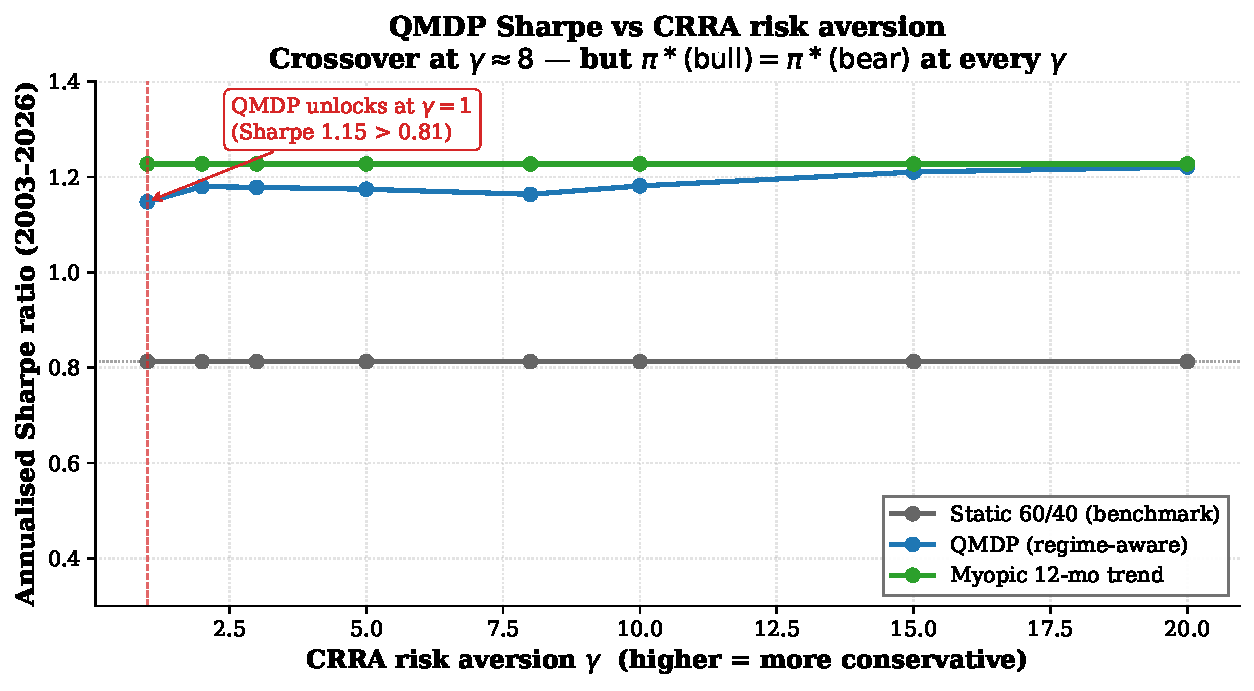
\includegraphics[width=\linewidth]{../figures/gamma_sensitivity_sharpe.pdf}
\caption{Annualised Sharpe vs.\ $\gamma$.}\label{fig:gamma-sharpe}
\end{subfigure}\hfill
\begin{subfigure}{0.48\linewidth}
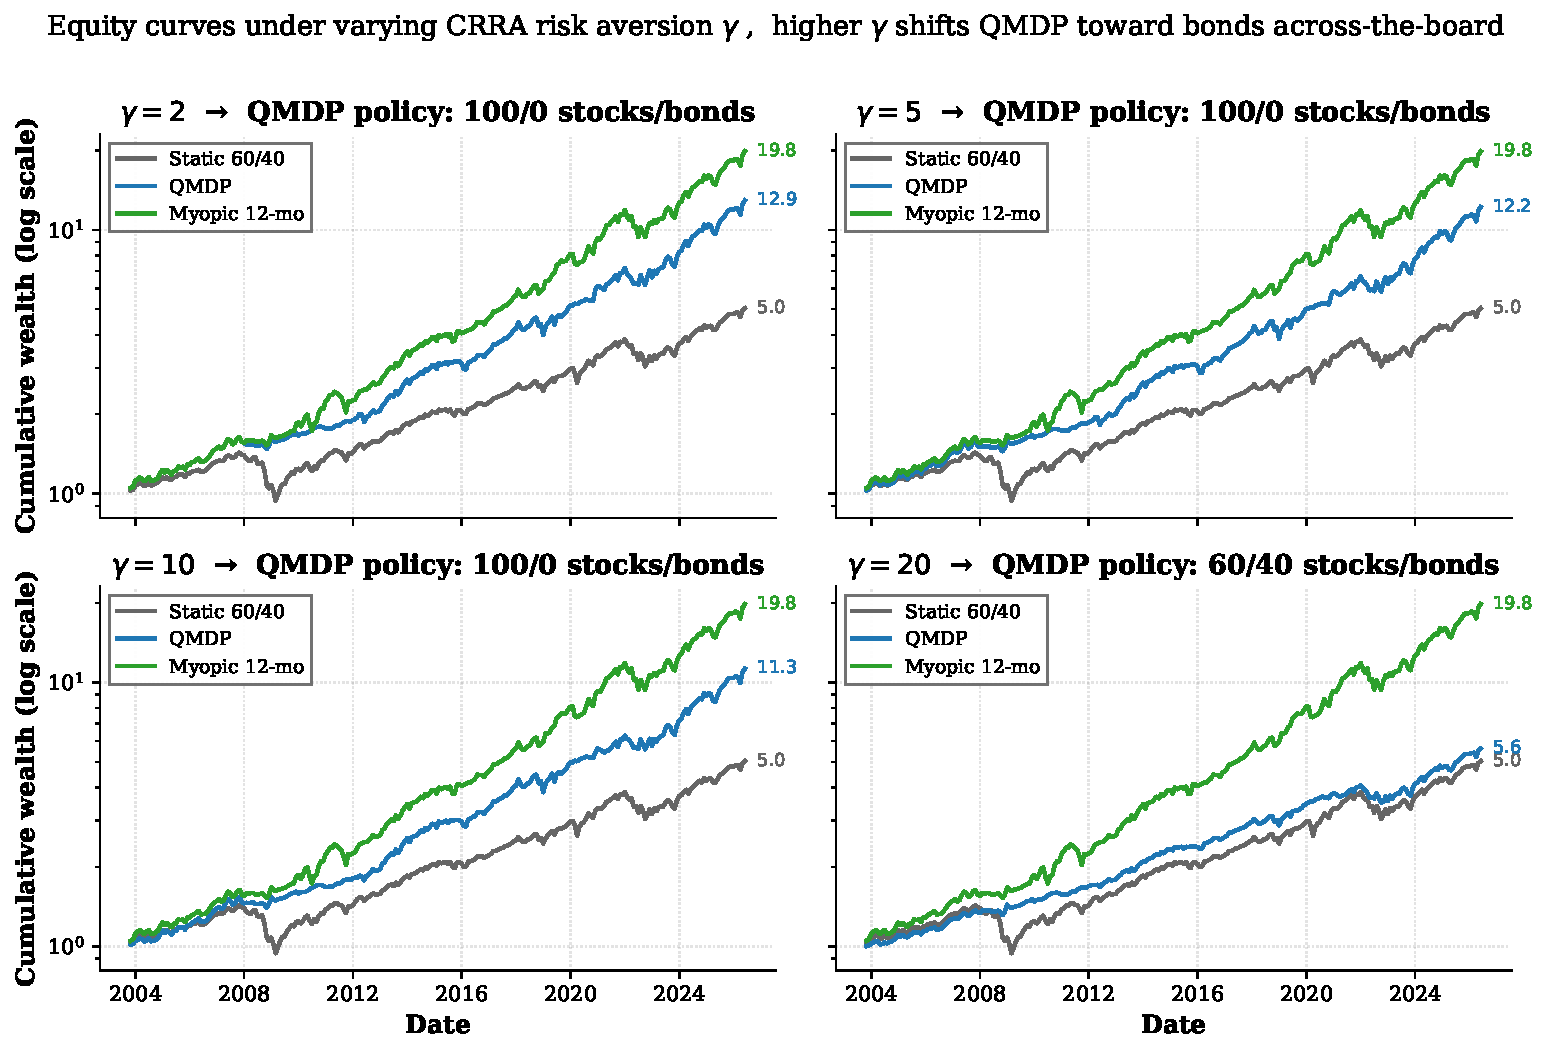
\includegraphics[width=\linewidth]{../figures/gamma_equity_curves.pdf}
\caption{Equity curves at $\gamma\in\{2,5,10,20\}$.}\label{fig:gamma-eq}
\end{subfigure}
\caption{CRRA risk-aversion sweep. Panel (a) plots the annualised Sharpe
ratio of each policy as $\gamma$ varies from 1 to 20. The static-60/40 and
myopic baselines are flat by construction. The QMDP Sharpe is below the
static benchmark for $\gamma\le 5$ and crosses above it at $\gamma=8$,
reaching $0.89$ by $\gamma\ge 15$. Panel (b) shows the corresponding
backtest equity curves at four representative $\gamma$ values. Each panel
title states the underlying MDP's optimal stock/bond split, illustrating
that higher risk aversion shifts the QMDP policy bondward across the
board, but never differentiates the bull and bear regimes.}\label{fig:gamma}
\end{figure}

\Cref{tab:gamma-policy} makes this concrete. Within each column the policy is
constant across rows (regime-insensitive), but it shifts \emph{column to
column} as $\gamma$ rises.

\begin{table}[t]
\centering
\caption{Optimal stock/bond split $\pi^\ast(s)$ as a function of regime $s$ and CRRA $\gamma$.
Within columns the two regimes give the \emph{same} action: the regime label does
not change the policy. The policy shifts \emph{across} columns as $\gamma$ rises.}
\label{tab:gamma-policy}
\small
\setlength{\tabcolsep}{6pt}
\renewcommand{\arraystretch}{1.1}
\begin{tabular}{lccccccc}
\toprule
Regime & $\gamma{=}1$ & $\gamma{=}2$ & $\gamma{=}3$ & $\gamma{=}5$ & $\gamma{=}8$ & $\gamma{=}15$ & $\gamma{=}20$ \\
\midrule
Bull (0) & 100/0 & 100/0 & 100/0 & 80/20 & 40/60 & 20/80 & 20/80 \\
Bear (1) & 100/0 & 100/0 & 100/0 & 80/20 & 40/60 & 20/80 & 20/80 \\
\bottomrule
\end{tabular}
\end{table}

%================================================
\section{Conclusions}\label{sec:conclusions}
%================================================

We built and stress-tested a POMDP-based regime overlay for stock-bond
allocation. The pipeline is correct (VI and PI agree numerically; the
2-state HMM cleanly recovers the major stress episodes; the QMDP control
is well-defined). At the same time, the headline backtest reveals a
qualitative finding worth taking seriously: \emph{the regime signal exists
in our observations but the regime action does not}, in the sense that the
optimal CRRA policy is the same in bull and bear regimes for every level of
risk aversion we tested. The Sharpe gain from raising $\gamma$ is a
"second-moment" effect: more risk aversion reduces equity exposure
across-the-board and therefore reduces drawdowns and volatility, but it
does not exploit the regime label.

\subsection*{Implications}

For a practitioner considering a regime-aware overlay, our results give
three concrete cautions. First, two macro observables (VIX and the term
spread) are not sufficient to differentiate the per-regime conditional
expected returns enough to drive a regime-dependent policy. Second, log
utility is too risk-tolerant: any case-study claiming gains from regime
switching under log utility is almost certainly capturing
\emph{higher mean exposure} rather than \emph{regime-aware tilting}. Third,
the most useful single comparator is not the static 60/40 but a \emph{myopic
trend-following baseline}, which captures recent first-moment information
without any latent-state machinery and was the highest-Sharpe policy we
tested.

\subsection*{Extensions}

We see three high-value extensions.

\emph{(i)~Richer observations.} The proposal called for ICE BofA HY OAS as
a third observation channel. Including HY OAS would reduce the spectral
overlap of the bull and bear emissions, plausibly producing regime-dependent
$\pi^\ast(s)$. Implementation requires a registered FRED API key, which
bypasses the public CSV truncation.

\emph{(ii)~Sharpe-style or CVaR-penalised reward.} A reward of the form
$R(s,\mathbf{a})=\E[\mathbf{a}^\top\mathbf{r}\mid s]-\kappa\Var[\mathbf{a}^\top\mathbf{r}\mid s]$
explicitly penalises bear-regime volatility and is more likely to produce a
regime-dependent policy. This is a one-line change in our reward module.

\emph{(iii)~Belief-space value iteration.} QMDP is the simplest belief-space
policy. Point-based value iteration~\cite{pineau2003} maintains an explicit
$\alpha$-vector representation and would, in principle, exploit information
value (the action of \emph{learning} the regime). On a 2-state model, the
belief simplex is a 1-D segment, so PBVI is cheap and worth running as a
diagnostic.

\subsection*{What this report demonstrates}

End-to-end, the project assembles a hidden Markov chain over regimes,
viewed through the lens of a Bayesian network, into a fully-observable
Bellman recursion solved by value iteration and cross-checked against exact
policy iteration, and wrapped in a belief-state controller via the QMDP
approximation. The natural model-free alternative, a multi-armed-bandit or
temporal-difference learner, is left to future work.

\bigskip
\hrule
\smallskip\noindent
\textbf{Reproducibility.} All code, data-fetching, intermediate artifacts,
and figures are committed to
\href{https://github.com/takakhoo/ENGS177_Final_Project}{\nolinkurl{takakhoo/ENGS177_Final_Project}}.
The end-to-end pipeline runs in under five minutes on a laptop.

%================================================
\begin{thebibliography}{99}
\bibitem{hamilton1989}
J.~D.~Hamilton.
\newblock A new approach to the economic analysis of nonstationary time series and the business cycle.
\newblock \emph{Econometrica}, 57(2):357--384, 1989.

\bibitem{ang2002}
A.~Ang and G.~Bekaert.
\newblock International asset allocation with regime shifts.
\newblock \emph{Review of Financial Studies}, 15(4):1137--1187, 2002.

\bibitem{guidolin2007}
M.~Guidolin and A.~Timmermann.
\newblock Asset allocation under multivariate regime switching.
\newblock \emph{Journal of Economic Dynamics and Control}, 31(11):3503--3544, 2007.

\bibitem{nystrup2018}
P.~Nystrup, H.~Madsen, and E.~Lindstr\"om.
\newblock Dynamic portfolio optimization across hidden market regimes.
\newblock \emph{Quantitative Finance}, 18(1):83--95, 2018.

\bibitem{kaelbling1998}
L.~P.~Kaelbling, M.~L.~Littman, and A.~R.~Cassandra.
\newblock Planning and acting in partially observable stochastic domains.
\newblock \emph{Artificial Intelligence}, 101(1--2):99--134, 1998.

\bibitem{littman1995}
M.~L.~Littman, A.~R.~Cassandra, and L.~P.~Kaelbling.
\newblock Learning policies for partially observable environments: scaling up.
\newblock \emph{Proc.~ICML 1995}, 362--370, 1995.

\bibitem{rabiner1989}
L.~R.~Rabiner.
\newblock A tutorial on hidden Markov models and selected applications in speech recognition.
\newblock \emph{Proceedings of the IEEE}, 77(2):257--286, 1989.

\bibitem{pineau2003}
J.~Pineau, G.~Gordon, and S.~Thrun.
\newblock Point-based value iteration: an anytime algorithm for POMDPs.
\newblock \emph{Proc.~IJCAI 2003}, 1025--1030, 2003.

\bibitem{puterman}
M.~L.~Puterman.
\newblock \emph{Markov Decision Processes: Discrete Stochastic Dynamic Programming}.
\newblock John Wiley \& Sons, 2005.

\bibitem{kochenderfer}
M.~J.~Kochenderfer.
\newblock \emph{Decision Making Under Uncertainty: Theory and Application}.
\newblock MIT Press, 2015.

\bibitem{sutton}
R.~S.~Sutton and A.~G.~Barto.
\newblock \emph{Reinforcement Learning: An Introduction}, 2nd ed.
\newblock MIT Press, 2018.

\bibitem{lopezdeprado}
M.~L\'opez~de~Prado.
\newblock \emph{Advances in Financial Machine Learning}.
\newblock John Wiley \& Sons, 2018.
\end{thebibliography}

\appendix
%================================================
\section{Team contributions}
%================================================

\noindent\small Contributions reported following the report-guidelines template.
Percentages indicate first-pass share; cross-review of all sections is by all
four members.

\begin{center}
\begin{tabular}{lcccc}
\toprule
Task & Dario & Even & Kyle (KDLL) & Taka \\
\midrule
Defined the problem & 25\% & 25\% & 25\% & 25\% \\
Collected data & 25\% & 25\% & 25\% & 25\% \\
Performed data analysis & 30\% & 20\% & 30\% & 20\% \\
Built model of uncertainty (HMM) & 70\% & 0\% & 20\% & 10\% \\
Built model of decision (POMDP) & 10\% & 30\% & 10\% & 50\% \\
Developed solution technique (VI/PI/QMDP) & 10\% & 60\% & 20\% & 10\% \\
Drafted initial report & 20\% & 20\% & 20\% & 40\% \\
Revised the report & 25\% & 25\% & 25\% & 25\% \\
Drafted initial slides & 25\% & 25\% & 25\% & 25\% \\
Revised the slides & 25\% & 25\% & 25\% & 25\% \\
\bottomrule
\end{tabular}
\end{center}

\end{document}
